    % -*- coding: utf-8 -*-
% --- Capítulo 4 ---

\chapter{Diseño y Arquitectura del Sistema}
\label{chap:diseno_arquitectura} 

Este capítulo describe la arquitectura global del sistema y las decisiones de diseño clave que guían su implementación. Los detalles técnicos completos de implementación se desarrollan en el Capítulo \ref{chap:implementacion}.

\section{Arquitectura General}
\label{sec:arquitectura_general}

El sistema sigue una arquitectura de microservicios, con un backend Flask que interactúa con una base de datos PostgreSQL/TimescaleDB y la API externa de Fitbit\textsuperscript{\textregistered}. La adquisición de datos se realiza mediante scripts Python independientes ejecutados por el planificador del sistema (`cron`). La Figura~\ref{fig:arquitectura_general} ilustra esta arquitectura.

\begin{figure}[htbp] 
    \centering
    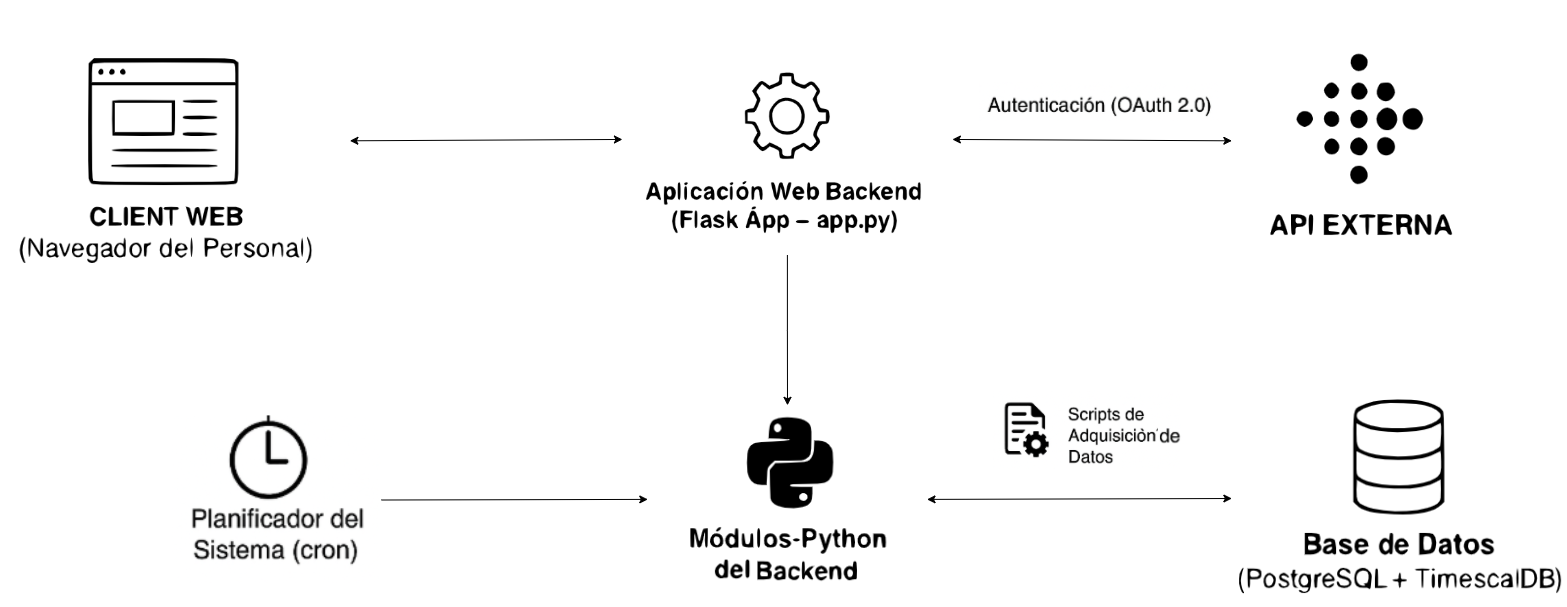
\includegraphics[width=0.9\textwidth]{imagenes/arquitectura_general.png}
    \caption{Arquitectura General del Sistema de Monitorización.}
    \label{fig:arquitectura_general}
\end{figure}

Los componentes principales y sus responsabilidades son:

\begin{itemize}
    \item \textbf{Cliente Web:} Interfaz HTML/CSS/JavaScript con visualizaciones Chart.js y soporte multilingüe.
    \item \textbf{Backend Flask:} Gestiona autenticación, vinculación de dispositivos y sirve el dashboard.
    \item \textbf{Scripts de Adquisición:} Procesos independientes para obtener datos de Fitbit.
    \item \textbf{Base de Datos:} PostgreSQL con TimescaleDB para series temporales.
\end{itemize}

\section{Diseño del Pipeline de Datos}
\label{sec:diseno_pipeline}

El pipeline de datos del sistema está diseñado para garantizar la adquisición, validación, almacenamiento y análisis eficiente de la información proveniente de los dispositivos Fitbit. El flujo se estructura en cinco componentes principales, como se ilustra en la Figura~\ref{fig:flujo_datos}:

\begin{enumerate}
    \item \textbf{Orquestación:} Scripts Python (\texttt{fitbit.py}, \texttt{fitbit\_intraday.py}) ejecutados periódicamente por \texttt{cron} para la adquisición automática de datos.
    \item \textbf{Adquisición:} Obtención de datos de la API de Fitbit mediante tokens OAuth 2.0 cifrados, con manejo robusto de errores y refresco automático de credenciales.
    \item \textbf{Almacenamiento:} Persistencia en hipertablas TimescaleDB optimizadas para series temporales (\texttt{daily\_summaries}, \texttt{intraday\_metrics}, \texttt{sleep\_logs}).
    \item \textbf{Procesamiento:} Evaluación automática de reglas de alerta basadas en umbrales científicos y patrones individuales, generando alertas clínicas cuando corresponde.
    \item \textbf{Visualización:} Interfaz web con dashboards interactivos para consulta, filtrado y exportación de datos y alertas.
\end{enumerate}

\begin{figure}[htbp]
    \centering
    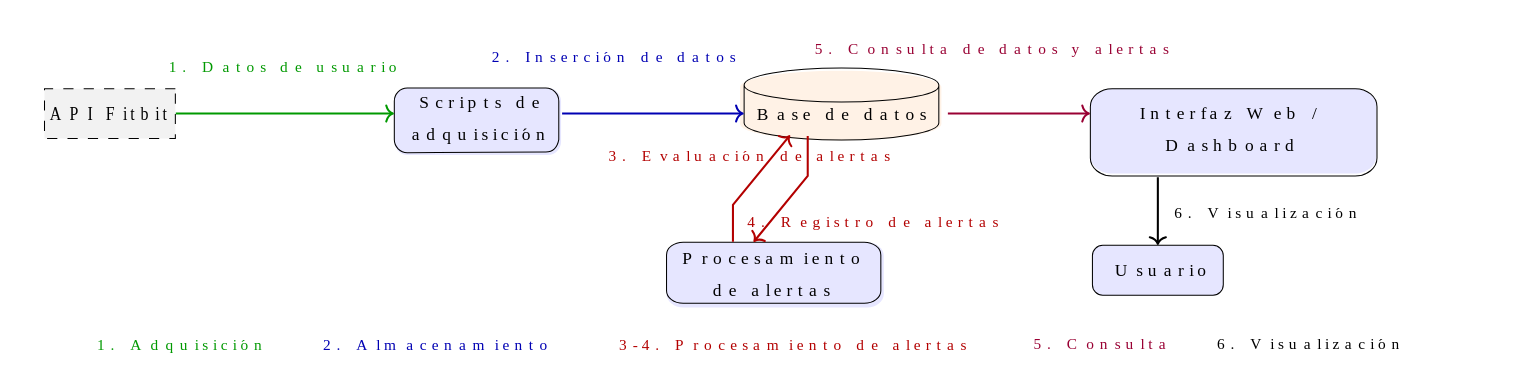
\includegraphics[width=1\textwidth, height=0.3\textheight]{imagenes/flujo_datos.png}
    \caption{Flujo de datos desde la API de Fitbit hasta la visualización en el dashboard.}
    \label{fig:flujo_datos}
\end{figure}

Este diseño modular desacopla la adquisición del análisis y la visualización, facilitando la escalabilidad y la integración futura de nuevas fuentes de datos o reglas de alerta. La evaluación de alertas se realiza de forma automática tras cada ingesta, comparando los datos recientes con líneas base individuales y umbrales predefinidos, almacenando los resultados en la tabla \texttt{alerts} para su posterior revisión clínica.(ver implementación en la Sección~\ref{subsec:anexo_actividad_drop}).

\subsection{Evaluación Dinámica de Reglas de Alerta}
La detección de anomalías y generación de alertas se realiza de forma automática tras cada ingesta de datos, mediante funciones desacopladas del frontend y definidas en un módulo específico. Las reglas pueden consultar ventanas temporales (por ejemplo, 7 días de pasos o sueño) y comparar los valores actuales con medias, umbrales o desviaciones estándar. El resultado se almacena en la tabla \texttt{alerts}, permitiendo su posterior revisión clínica.

El diseño modular facilita la incorporación de nuevas reglas, la extensión a patrones más complejos o incluso la integración futura de algoritmos de aprendizaje automático.


\section{Diseño del Backend (Aplicación Flask y Scripts)}
\label{sec:diseno_backend}

El backend se estructura en dos componentes principales:

\begin{enumerate}
    \item \textbf{Aplicación Web Flask:} 
        \begin{itemize}
            \item Servir las páginas HTML para el login, la selección de email, la asignación de nombre y las confirmaciones (usando plantillas Jinja2 multilenguaje).
            \item Gestionar el flujo OAuth 2.0: generar parámetros (`state`, `code\_challenge`), construir la URL de autorización, manejar la redirección del usuario a Fitbit\textsuperscript{\textregistered} y procesar el `callback`.
            \item Interactuar con \texttt{auth.py} para obtener los tokens a partir del código de autorización.
            \item Interactuar con \texttt{db.py} y \texttt{encryption.py} para guardar/actualizar la información del usuario y los tokens cifrados en la tabla \texttt{users}.
            \item Servir el dashboard y exponer endpoints API para la precarga y actualización eficiente de datos, optimizando la latencia y la escalabilidad. La implementación de las rutas principales se detalla en la Sección~\ref{subsec:anexo_rutas} del Anexo.
            \item Gestionar logs y errores de forma centralizada para garantizar la robustez del sistema.
        \end{itemize}
    \item \textbf{Scripts de Adquisición:} 
        \begin{itemize}
            \item Obtiene y descifra los tokens (\texttt{encryption.py}, \texttt{db.py}).
            \item Verifica la validez del token de acceso (\texttt{expires\_at}). Si es necesario, intenta refrescarlo usando el token de refresco (\texttt{auth.py}, \texttt{fitbit.py}) y actualiza los tokens cifrados y la expiración en la BD (\texttt{db.py}).
            \item Si los tokens son válidos, realiza las llamadas correspondientes a la API de Fitbit\textsuperscript{\textregistered} (\texttt{fitbit.py}, \texttt{fitbit\_intraday.py}).
            \item Procesa la respuesta JSON y maneja posibles errores, registrando los fallos y continuando con el siguiente usuario para garantizar la robustez.
            \item Se conecta a la BD (\texttt{db.py}) para insertar los datos procesados en las tablas/hipertablas de TimescaleDB apropiadas.
            \item Tras la inserción, ejecuta la lógica de evaluación de alertas de forma desacoplada, permitiendo la extensión futura a reglas más complejas o nuevos tipos de datos.
        \end{itemize}
\end{enumerate}
Esta separación y modularidad permiten que la adquisición de datos no bloquee la aplicación web, facilitan la escalabilidad (añadiendo más scripts o fuentes de datos) y mejoran la mantenibilidad del sistema.

\section{Diseño de la Base de Datos (PostgreSQL + TimescaleDB)}
\label{sec:diseno_bd}

La base de datos combina PostgreSQL con la extensión TimescaleDB para optimizar el manejo de series temporales. La Figura~\ref{fig:esquema_relacional} muestra el esquema completo.

\begin{figure}[htbp]
    \centering
    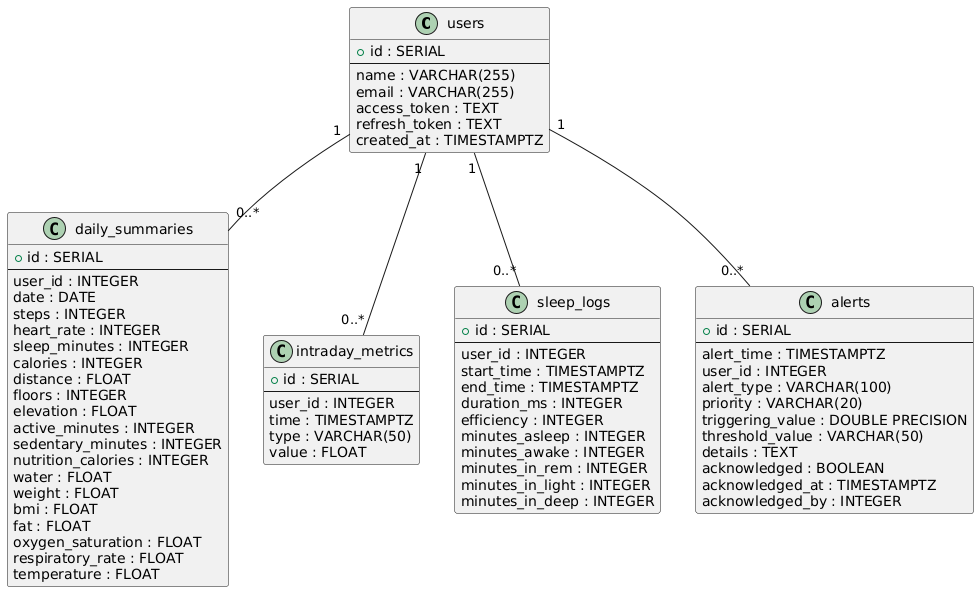
\includegraphics[width=0.9\textwidth]{imagenes/esquema_relacional.png}
    \caption{Esquema relacional de la base de datos del sistema.}
    \label{fig:esquema_relacional}
\end{figure}

El modelo se estructura en:
\begin{itemize}
    \item \textbf{Tabla Relacional:} \texttt{users} para gestión de usuarios y tokens
    \item \textbf{Hipertablas TimescaleDB:} Para datos temporales (métricas diarias, intradía, sueño y alertas)
\end{itemize}

Las sentencias SQL detalladas y la descripción de campos se encuentran en el Anexo~\ref{app:db_schema}.


\section{Diseño de la Interfaz de Usuario}
\label{sec:diseno_ui}

La interfaz de usuario (UI) del sistema está diseñada para ser intuitiva, accesible y eficiente con soporte multilingüe (español/inglés) facilitando tanto la gestión administrativa como la visualización clínica de los datos monitorizados. Se compone de dos grandes bloques:

\begin{itemize}
    \item \textbf{Interfaz de Gestión y Vinculación (Flask/HTML + Bootstrap):}
        \begin{itemize}
            \item Login y gestión de dispositivos
            \item Flujo OAuth 2.0 para vinculación
            \item Soporte multilingüe (ES/EN)
        \end{itemize}
    \item \textbf{Dashboard de Visualización y Alertas:}
        \begin{itemize}
            \item Implementado como un conjunto de vistas Flask con plantillas Jinja2 y componentes interactivos (JavaScript, Chart.js).
            \item Permite visualizar resúmenes diarios, métricas intradía, patrones de sueño y alertas recientes para cada usuario.
            \item Incluye filtros avanzados (por usuario, fecha, tipo de alerta, prioridad, etc.) y opciones de exportación a CSV.
            \item La precarga de datos y la optimización de consultas mejoran la velocidad de carga y la experiencia de usuario, especialmente en el dashboard de alertas. La implementación de las llamadas AJAX para la actualización dinámica se muestra en la Sección~\ref{subsec:anexo_formularios} del Anexo.
        \end{itemize}
\end{itemize}

El diseño modular y el uso de tecnologías estándar (Flask, Bootstrap, Chart.js) facilitan el mantenimiento y la extensión del sistema, mientras que la internacionalización integrada mejora la accesibilidad para usuarios de diferentes regiones.

\subsection{Ficha de Usuario y Visualización Individual}
Una de las vistas más relevantes del sistema es la \textbf{ficha de usuario} (\texttt{user\_detail.html}), que centraliza toda la información relevante de cada paciente o usuario monitorizado. Esta vista está diseñada para facilitar la toma de decisiones clínicas y el seguimiento personalizado, integrando:

\begin{itemize}
    \item \textbf{Resumen de datos personales:} nombre, email, fecha de registro y estado de actividad reciente.
    \item \textbf{Métricas clave del día:} pasos, frecuencia cardíaca, horas de sueño, calorías, etc., resaltando visualmente cualquier valor anómalo o alerta activa.
    \item \textbf{Alertas recientes:} listado de alertas generadas en los últimos días, con posibilidad de reconocerlas directamente desde la ficha.
    \item \textbf{Gráficos interactivos:} evolución semanal de pasos, sueño, frecuencia cardíaca y minutos activos, así como visualización intradía y análisis de patrones de inactividad, implementados con Chart.js.
    \item \textbf{Tabs de navegación:} acceso rápido a diferentes vistas (resumen diario, intradía, semanal, alertas, inactividad).
    \item \textbf{Exportación y actualización:} botones para exportar datos a CSV y actualizar la información en tiempo real.
    \item \textbf{Accesibilidad y usabilidad:} diseño responsivo, iconografía clara, leyendas de colores para priorización y mensajes de estado.
\end{itemize}

Esta ficha ejemplifica la integración de todos los módulos del sistema (adquisición, almacenamiento, análisis y visualización), permitiendo al personal sanitario o gestor acceder de forma rápida y comprensible a la información más relevante para cada usuario.

\subsection{Diseño del Módulo de Alertas}
\label{subsec:diseno_alertas}

El módulo de alertas es un componente central del sistema, encargado de analizar los datos almacenados y detectar automáticamente situaciones clínicas relevantes o anomalías en la actividad, el sueño o la frecuencia cardíaca de los usuarios. Su diseño es modular y desacoplado del frontend, permitiendo su ejecución periódica tras cada ingesta de datos y facilitando la extensión futura con nuevas reglas o métricas.

\begin{itemize}
    \item \textbf{Acceso a datos históricos:} El módulo dispone de funciones específicas (en \texttt{db.py}) para recuperar las métricas necesarias en ventanas temporales (por ejemplo, los últimos 7 días de pasos o sueño) y realizar comparaciones con la línea base individual de cada usuario.
    \item \textbf{Lógica de comparación y reglas:} Las reglas de alerta están implementadas en Python (\texttt{alert\_rules.py}) y se basan en umbrales científicos, porcentajes de cambio, desviaciones estándar o rangos fisiológicos. Cada función evalúa si los datos actuales superan los límites definidos y, en caso afirmativo, genera una alerta con prioridad, tipo, valor disparador y detalles clínicos.
    \item \textbf{Registro y gestión de alertas:} Las alertas detectadas se almacenan en la tabla \texttt{alerts}, asociando cada evento con el usuario, la métrica, la prioridad y una descripción. Esto permite su posterior visualización, filtrado y exportación desde el dashboard.
    \item \textbf{Extensibilidad:} El diseño permite añadir fácilmente nuevas reglas, métricas o fuentes de datos, así como adaptar los umbrales según la evidencia clínica o la experiencia práctica.
\end{itemize}

\subsubsection{Manejo de Datos Faltantes o Erróneos}
La calidad de los datos de wearables puede verse afectada por desconexiones, falta de uso o errores de medición. El sistema implementa estrategias robustas para minimizar falsas alarmas y garantizar la fiabilidad de las alertas:
\begin{itemize}
    \item Se requiere un porcentaje mínimo de días con datos válidos en las ventanas temporales para evaluar una alerta (por ejemplo, al menos 5 de 7 días).
    \item Se aplican filtros de rango fisiológico antes de procesar los datos (por ejemplo, descartar valores de frecuencia cardíaca fuera de 30-200 bpm o pasos diarios superiores a 50.000).
    \item Los datos faltantes críticos generan alertas de calidad de datos, permitiendo al personal identificar posibles problemas de uso o sincronización.
\end{itemize}

\subsubsection{Optimización y Rendimiento}
Dado el volumen potencial de datos y la necesidad de evaluaciones históricas frecuentes, el sistema optimiza el acceso y procesamiento mediante:
\begin{itemize}
    \item Índices compuestos en las hipertablas de TimescaleDB (por ejemplo, sobre \texttt{(user\_id, time)}) para acelerar las consultas.
    \item Cálculos eficientes en los scripts, reutilizando los datos recuperados para varias métricas cuando es posible.
    \item Procesamiento asíncrono y desacoplado mediante la ejecución periódica por \texttt{cron}, evitando que la evaluación de alertas afecte la experiencia de usuario en la interfaz web.
\end{itemize}

\subsubsection{Diagrama de Flujo del Proceso de Detección de Alertas}
El proceso lógico para la detección y registro de alertas sigue el flujo ilustrado en la Figura~\ref{fig:diagrama_alertas}:

\begin{figure}[htbp]
    \centering
    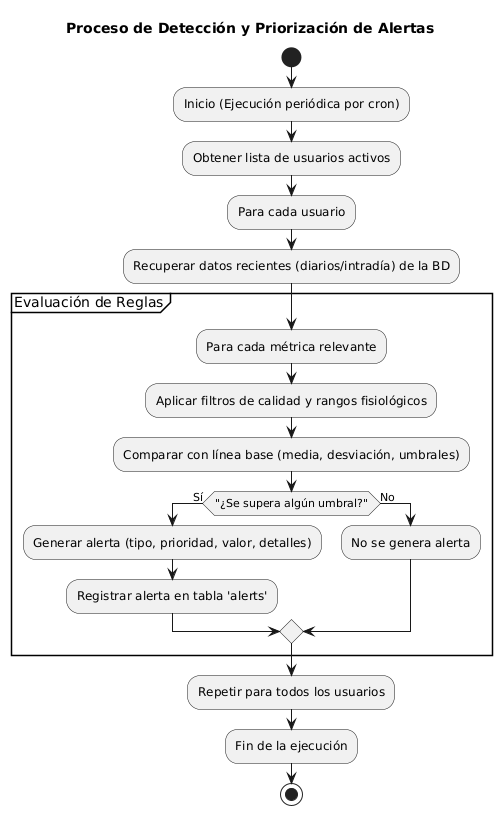
\includegraphics[width=0.9\textwidth,height=0.6\textheight]{imagenes/diagrama_alertas.png} 
    \caption{Diagrama de flujo del proceso de detección y priorización de alertas.}
    \label{fig:diagrama_alertas}
\end{figure}

Este diseño permite que la evaluación de alertas se beneficie de las optimizaciones de consulta de TimescaleDB y se mantenga desacoplada de la interfaz de usuario, garantizando robustez, escalabilidad y relevancia clínica.
Los umbrales detallados y su justificación se documentan en el Anexo~\ref{anexo:anexo_umbrales}.

\subsection{Arquitectura de la Interfaz Web y Dashboards}
\label{sec:arquitectura_dashboard}

La interfaz web del sistema está compuesta por dos dashboards principales:

\begin{itemize}
    \item \textbf{Dashboard de Alertas:} Permite al personal autorizado visualizar, filtrar y exportar todas las alertas generadas por el sistema. Incluye filtros por fecha, usuario, tipo de alerta, prioridad y estado de reconocimiento. Cada alerta puede ser reconocida manualmente y se muestra información detallada, incluyendo datos intradía relevantes y contexto clínico.
    \item \textbf{Dashboard de Usuarios:} Presenta un listado de todos los usuarios monitorizados, con búsqueda por nombre o email y estado de actividad reciente. Desde aquí se accede a la ficha de usuario.
\end{itemize}

La \textbf{ficha de usuario} incluye:
\begin{itemize}
    \item Resumen diario de métricas clave (pasos, frecuencia cardíaca, sueño, calorías, etc.).
    \item Visualización de datos intradía (gráficos de pasos, FC, calorías, minutos activos).
    \item Resumen semanal (tendencias de pasos, sueño, actividad, etc.).
    \item Listado de alertas recientes y posibilidad de exportarlas.
    \item Análisis de patrones de inactividad (detección de periodos prolongados sin actividad).
    \item Exportación de datos históricos e intradía en formato CSV.
\end{itemize}

La navegación entre dashboards y fichas de usuario es intuitiva y está protegida por autenticación. El diseño prioriza la claridad visual y la accesibilidad para facilitar la toma de decisiones clínicas.
